\documentclass[../main.tex]{subfiles}
\graphicspath{{\subfix{../figures/}}}

\begin{document}
\section{组合/聚合复用原则(CARP)}
Composition/Aggregation Reuse Principle

组合、聚合复用原则就是在一个新的对象里面应尽量使用一些已有的对象,使之成为新对象的一部份,新的对象通过向这些对象的委派达到复用已有功能的目的。
这个原则有一个简短的描述:要尽量使用组合、聚合,尽量不要使用继承。

\noindent \textbf{组合与聚合的区别}:组合和聚合均是关联的特殊情形。
聚合:拥有关系或整体与部分的关系;
组合:一种强得多的拥有关系;

\textbf{复用的基本种类}:在面向对象的设计里,有两种基本的方法可以在不同的环境中复用已有的设计和实现,即通过组合/聚合或继承。

\noindent \textbf{组合/聚合复用的优点}:
\begin{itemize}
  \item 组合/整体对象存取成分/部分对象的唯一方法是通过成分/部分对象的接口。
  \item 这种复用是黑箱复用,因为成分对象的内部细节是新对象所看不见的,容易实现封装。
  \item 这种复用所需的依赖较少。
  \item 这种复用可以在运行时间内动态进行,新对象可以动态的引用与成分对象类型相同的其它对象。
\end{itemize}
\noindent \textbf{组合/聚合复用的缺点}:
采用这种复用关系的系统会有较多的对象需要管理。

\noindent \textbf{继承复用的优点}:实现新的子类较为容易,因为超类的大部分功能可以通过继承关系自动进入子类。
修改和扩展继承而来的实现较为容易。

\noindent \textbf{继承复用的缺点}:
\begin{itemize}
  \item 继承复用破坏封装,因为继承将超类的实现细节暴露给子类。由于超类的内部细节常常是对于子类透明的,所以这种复用是透明的复用,又称“白箱”复用。
  \item 如果超类发生改变,那么子类的实现也不得不发生改变。
  \item 从超类继承而来的实现是静态的,不可能在运行时间内发生改变,没有足够的灵活性。
\end{itemize}

\textbf{区分``Is-A''和``Has-A''}:
\begin{itemize}
  \item ``Is-A''代表一个类是另外一个类的一种
  \item ``Has-A''代表一个类是另一个类的一个部分,而不是另一个类的特殊种类。
  \item 对于``Is-A''应该考虑使用继承,而``Has-A''使用组合/聚合。
\end{itemize}
应当采用组合/聚合的例子:
\begin{figure}[H]
  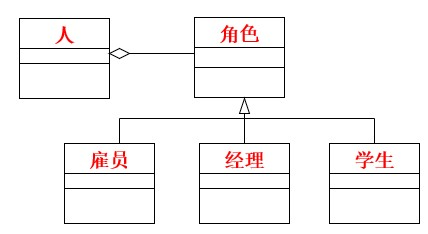
\includegraphics[width=0.55\textwidth]{13_1.jpg}
\end{figure}
\textbf{与里氏代换原则联合使用}:
\begin{itemize}
  \item 里氏代换原则是继承复用的基石。只有当派生类可以替换掉基类,软件模块的功能不会受到影响时,基类才真正被复用,而派生类也才能够在基类的基础上增加新的功能。
  \item 如果两个类的关系是``Has-A''而不是``Is-A''关系,这两个类一定违反里氏代换原则。
  \item 只有两个类满足里氏代换原则,才有可能是``Is-A''关系。
\end{itemize}
\end{document}
